\textbf{Do heads succeed together?} On 13,602 training and validation states, the marginal product predicted a 14.30\% hit rate for the path taking the top rank in heads one and two. The observed rate was 19.66\% (2,674 hits), or 1.37 times the product estimate. The second head's marginal top-rank accuracy was 28.39\%. Conditional on a first-head top-rank hit, it reached 39.03\% across 6,852 surviving prefixes. The analogous third-head rates were 17.96\% and 37.55\%. The fifth head reached 47.41\% conditional accuracy, but only 424 prefixes survived to that comparison. The dependence is strongest on some paths and leaves fewer examples for estimating deeper factors.

\paragraph{Equal-budget comparison.} Each policy selects the same number of nonroot nodes. All 80 evaluation questions contributed, with a median of 59 complete states per question and a range of 1 to 59. The last two columns of Table~\ref{tab:replay} refer to a shared path pool and are independent of budget.
\begin{table}[ht]\centering
\caption{Mean committed tokens per eligible MT-Bench state at five draft budgets. The final columns report path prediction error (lower is better).}\label{tab:replay}
\begin{center}
\begin{tabular}{lrrrrrrr}
\toprule
Policy & 8 & 16 & 32 & 63 & 96 & Brier & ECE\\
\midrule
Fixed marginal & 2.106 & 2.314 & 2.486 & 2.634 & 2.704 & 0.02126 & 0.00643\\
Fixed conditional & 2.150 & 2.342 & 2.516 & 2.653 & 2.725 & 0.02112 & 0.00441\\
MEDUSA+ & 2.268 & 2.452 & 2.604 & 2.726 & 2.792 & 0.01839 & 0.00135\\
Direct classifier & 2.269 & 2.455 & 2.605 & 2.730 & 2.791 & 0.01842 & 0.00172\\
Dynamic conditional & 2.268 & 2.451 & 2.607 & 2.731 & 2.794 & 0.01845 & 0.00125\\
\bottomrule
\end{tabular}
\end{center}

\end{table}

The fixed conditional tree gained the most at $B=8$, from 2.106 to 2.150 tokens per state (2.10\%). Its improvement persisted at $B=63$ ($+0.0192$, 95\% paired interval $[0.0063,0.0341]$). MEDUSA+ exceeded both fixed trees at every budget. With 63 nodes, fitting conditional factors changed dynamic acceptance from 2.7264 to 2.7306 ($+0.0042$, interval $[-0.0009,0.0090]$). The direct classifier reached 2.7299.
\begin{figure}[ht]\centering
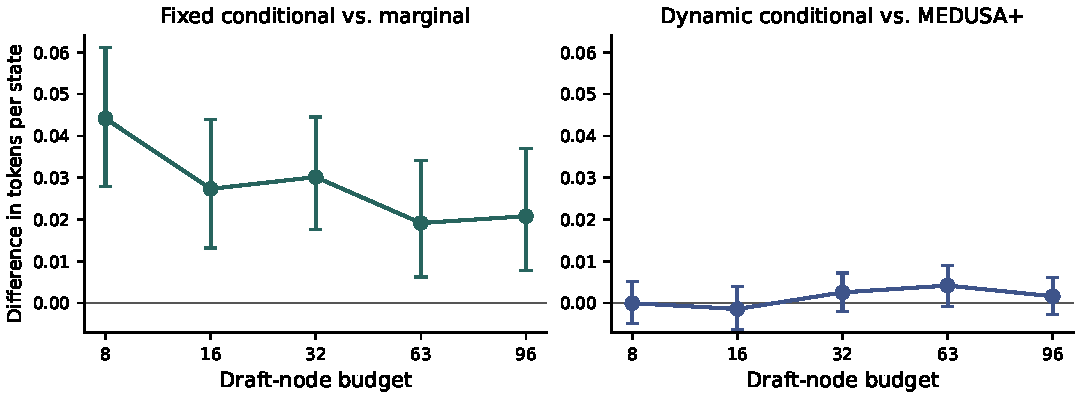
\includegraphics[width=.96\linewidth]{tables/paired_acceptance.pdf}
\caption{Change in accepted tokens at equal budgets. Bars are per-budget 95\% paired prompt-bootstrap intervals on the same vertical scale. Every fixed contrast favors conditioning. The dynamic contrasts each admit gains and losses.}
\end{figure}
Increasing the budget from 63 to 96 adds 33 draft nodes. Even the best observed mean increases by only about 0.06 tokens per eligible state over that range. This diminishing return motivates measuring the cost of wider verification directly.
